
\section{City-folding Visual Analytics}

Semantic understanding of social characteristics.

\subsection{Data-driven Visual Profile}

Glyph design is 

to abstract to concrete and semantic understanding, to help users clues to do the classification. 

Face... Data-driven inforgraphics~\cite{}. Following the idea of Chernoff Face~\cite{1973}, we utilize that we better know the perceptual figures well before we use them. By designing different visual dimensions, knowned as a type of glyph, a graphical representation of people with specific social characteristics. Those visual profiles are intended for intutive visual understanding and clustering. 

Figure~\ref{fig:design_profile} shows the legend for the user profile. Those design dimensions are driven by data. an intuitive perception of the social characteristics. 

Considering the driven machinsm in two attributes: 
\begin{itemize}
\item \textit{Numerical}
\item \textit{Categorical}
\end{itemize}

\begin{figure}[htb!]
 \centering % avoid the use of \begin{center}...\end{center} and use \centering instead (more compact)
 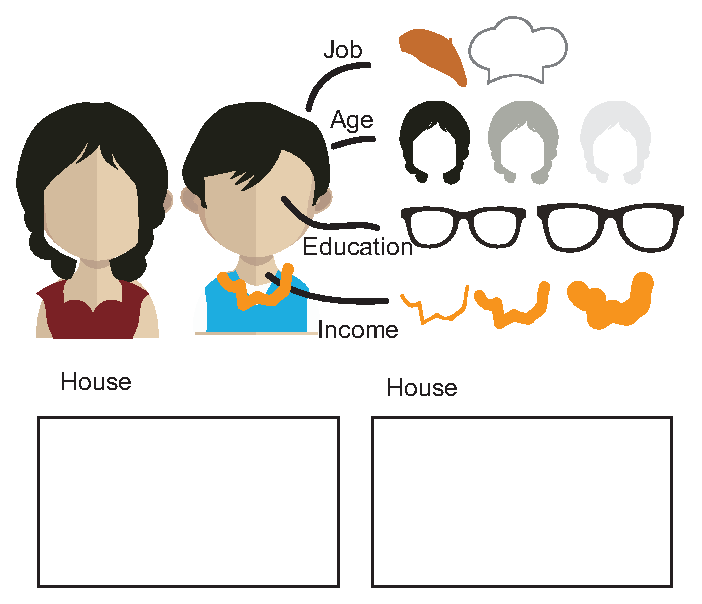
\includegraphics[width=\columnwidth]{pictures/design_profile}
 \caption{Design Profile}
 \label{fig:design_profile}
\end{figure}

Various profiles are generated. Figure~\ref{fig:div_profile} shows some results.

\begin{figure}[htb!]
 \centering % avoid the use of \begin{center}...\end{center} and use \centering instead (more compact)
 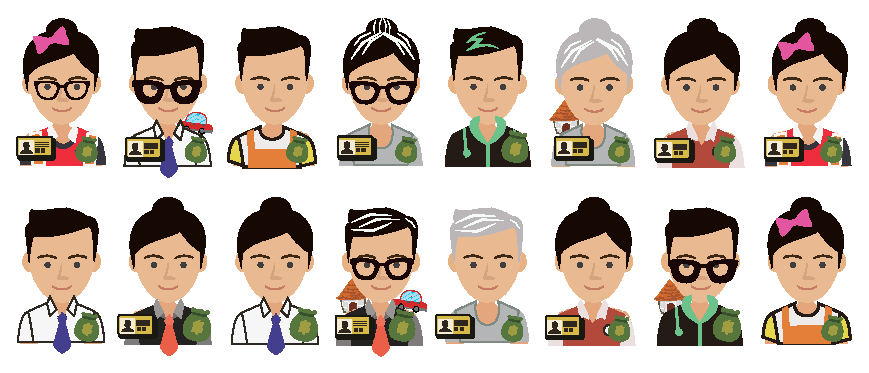
\includegraphics[width=\columnwidth]{pictures/design_div}
 \caption{Diverse Profile}
 \label{fig:div_profile}
\end{figure}

\subsection{Interactive Group Classification}

Figure~\ref{fig:mds} is the MDS project of diversse users. Contour detected. Classification Updated. Automatic ensembling of diverse profiles. 

Groups from demographics

\begin{figure}[htb!]
 \centering % avoid the use of \begin{center}...\end{center} and use \centering instead (more compact)
 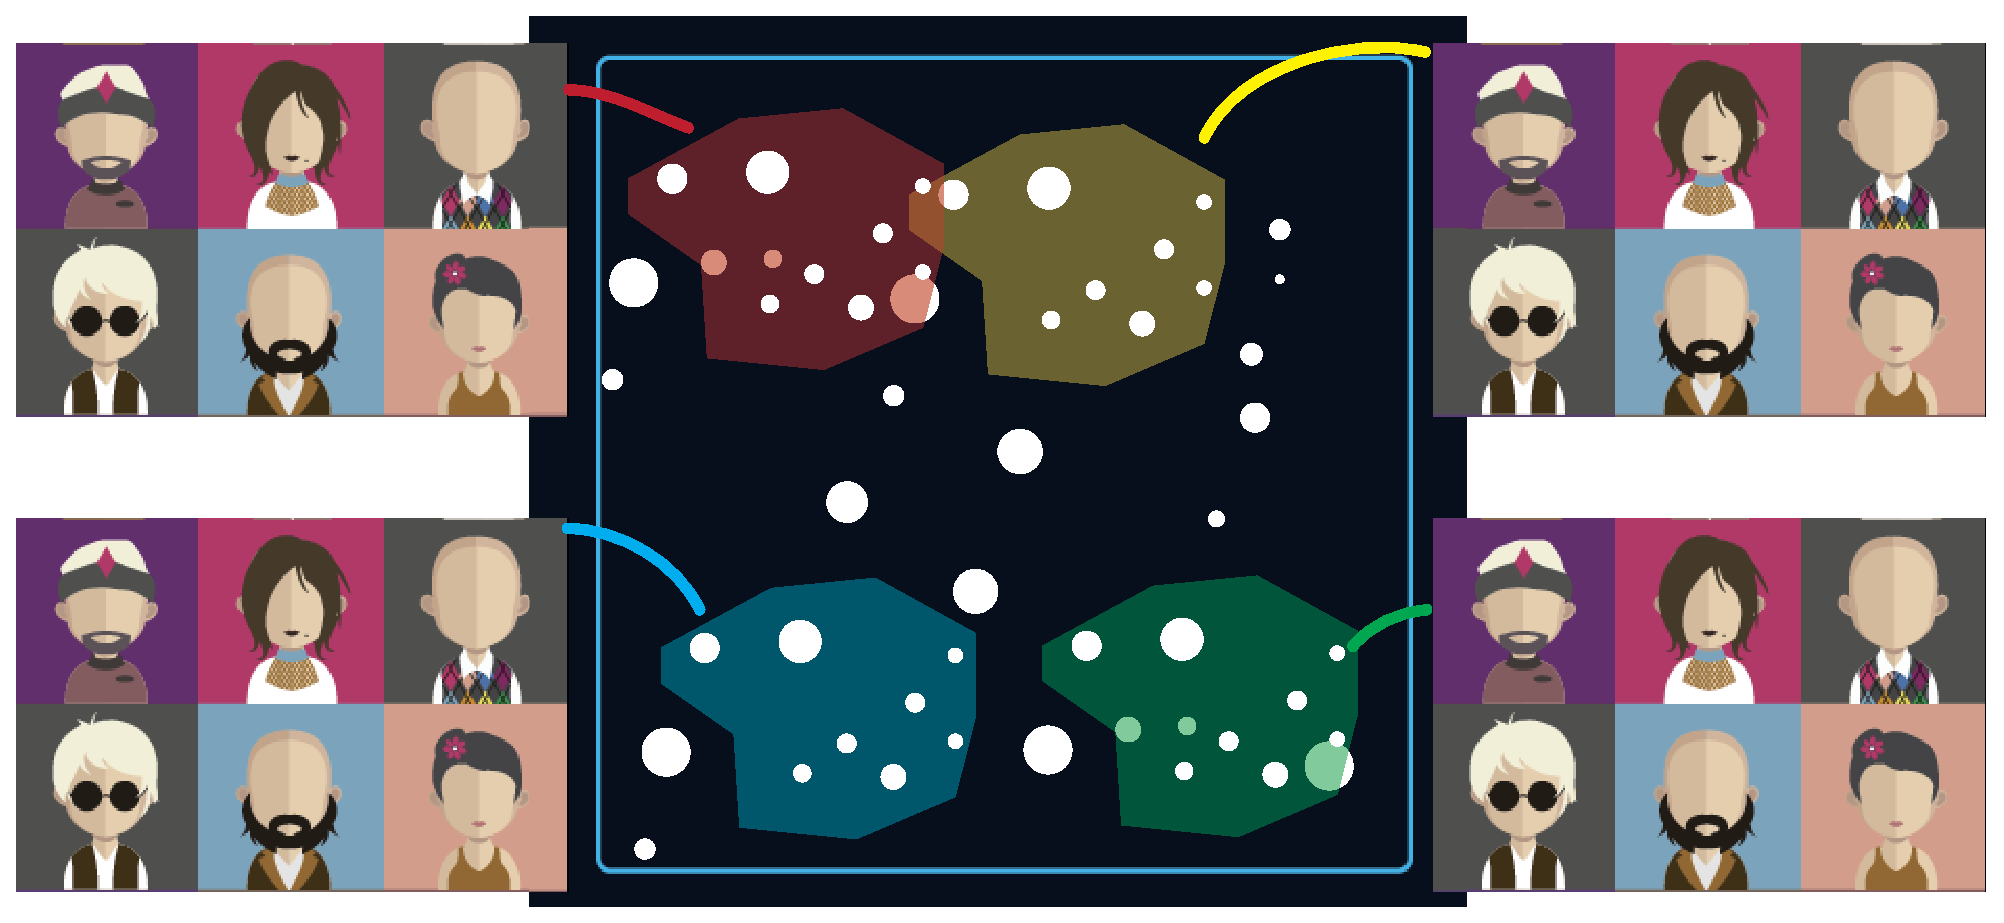
\includegraphics[width=\columnwidth]{pictures/mds}
 \caption{Interactive Labelling and Classification}
 \label{fig:mds}
\end{figure}

\subsection{Spatial Visualization}

The space visualization is embedded in 2.5D space. TAZ is used as the .... The height of space is put as the occurrence of visiting. For each group of people, we adjust the DB-Scan Algorithm in the context of TAZ. 